\documentclass[runningheads]{llncs}
\usepackage[T1]{fontenc}
\usepackage{lmodern}
\usepackage{graphicx}
\usepackage{array}
\usepackage{float}
\usepackage{longtable}
\usepackage{xurl}
\usepackage[protrusion=false]{microtype}
\usepackage{tikz}
\usetikzlibrary{arrows.meta,positioning,shapes.geometric}
% Frozen post-fit metrics from the selected matched build pair.
\newcommand{\BaselineLE}{347}
\newcommand{\BaselineReg}{216}
\newcommand{\BaselineFmax}{123.00}
\newcommand{\SecureLE}{5655}
\newcommand{\SecureLEPrint}{5,655}
\newcommand{\SecureReg}{917}
\newcommand{\SecureFmax}{95.07}
% xurl permits breaks throughout each hash without changing its characters.
\urlstyle{tt}
\newcommand{\SHA}[4]{\path{#1#2#3#4}}
\newcolumntype{P}[1]{>{\raggedright\arraybackslash}p{#1}}
% Match the LNCS caption style for the table that can span pages.
\makeatletter
\renewcommand{\LT@makecaption}[3]{%
  \LT@mcol\LT@cols c{\hbox to\z@{\hss
    \parbox[t]{\LTcapwidth}{%
      \small
      \sbox\@tempboxa{#1{\textbf{#2.} }#3}%
      \ifdim\wd\@tempboxa>\hsize
        #1{\textbf{#2.} }#3\par
      \else
        \hbox to\hsize{\hfil\box\@tempboxa\hfil}%
      \fi
      \vskip6pt
    }\hss}}%
}
\makeatother
\renewcommand{\arraystretch}{1.12}
\setlength{\tabcolsep}{4pt}
\setcounter{secnumdepth}{2}
% Give difficult justified lines additional room to adjust their spacing.
\setlength{\emergencystretch}{2em}
% Avoid large vertical gaps from flush-bottom stretching on sparse pages.
\raggedbottom

\begin{document}

\title{Hardware Cost and Live GPS Data-Path Evaluation of AES-128-CTR on an FPGA}
\titlerunning{AES-CTR for Live GPS Data on an FPGA}
\author{Cavalcante, L. F.\inst{1}\orcidID{0009-0000-0216-5157}\thanks{Corresponding author: lfc.eng23@uea.edu.br.} \and
Santos, I. T. F.\inst{1}\orcidID{0009-0004-6900-957X} \and
Amaral, F. E.\inst{1}\orcidID{0009-0006-3116-9601} \and
Fernandes, B. G.\inst{1}\orcidID{0009-0008-8963-4275} \and
Silva, E. L. O.\inst{1}\orcidID{0000-0003-2722-2191}}
\authorrunning{L. F. Cavalcante et al.}
\institute{
Laborat\'orio de Sistemas Digitais e Microeletr\^onica (LSD$\mu$)\\
Escola Superior de Tecnologia (EST)\\
Universidade do Estado do Amazonas (UEA),\\
Manaus, Brazil\\
\email{\{lfc.eng23,itfds.eng20,feda.eng23,bgfe.eng24,elsilva\}@uea.edu.br}
}

\maketitle

\begin{abstract}
GPS receivers commonly expose navigation messages through UART, which does not provide confidentiality. This paper evaluates the hardware cost and live data-path behavior of adding AES-128 in counter mode (CTR) to a GPS UART stream on a DE10-Lite/MAX 10 FPGA. Matched baseline and AES-CTR builds share a 50~MHz clock, 9600/8N1 serial interface, 1,024-byte FIFO, device, and timing constraints. The selected post-fit baseline uses \BaselineLE{} logic elements (LEs) and \BaselineReg{} registers; the AES-CTR design uses \SecureLEPrint{} LEs and \SecureReg{} registers. Their minimum Fmax values are \BaselineFmax{} and \SecureFmax{}~MHz, respectively, and both meet the 50~MHz operating constraint with positive setup, hold, recovery, and removal slack. Simultaneous live GPS trials showed exact baseline forwarding and exact recovery after AES-CTR for matched 1,024-byte captures, each containing 24 checksum-valid NMEA sentences. A separate 65,536-byte AES-CTR live capture was also recovered byte-exactly, including 1,112 complete valid NMEA sentences. AES-CTR provides confidentiality but not authentication; key provisioning and nonce lifecycle remain deployment requirements. Overall, the evaluated datapath preserved live GPS bytes while meeting the target's 50~MHz timing constraint.
\keywords{FPGA \and AES-128-CTR \and GPS \and UART \and NMEA \and Hardware evaluation}
\end{abstract}

\section{Introduction}
Navigation receivers often expose position and timing messages over an asynchronous serial interface. NMEA sentences are convenient to integrate, but a UART link does not conceal their contents. Adding encryption in programmable logic therefore raises a practical engineering question: what hardware cost accompanies confidentiality processing on a small FPGA, and can the live sensor-to-host path preserve the input bytes?

This work compares two otherwise matched UART datapaths on a DE10-Lite/MAX 10. The baseline forwards bytes; the AES-CTR variant adds the cipher transform. Both operate at 50~MHz, 9600 baud with 8N1 framing, and use a 1,024-byte FIFO. A u-blox NEO-M8N supplies live NMEA data. An Analog Discovery 2 (AD2) samples the GPS input and FPGA output simultaneously, while a CP2102 provides an independent host-side serial copy. An independent software implementation decrypts the captured ciphertext and compares all recovered bytes with the concurrent GPS reference.

The study asks (1) how AES-CTR changes post-fit logic, register use, and timing under matched constraints, and (2) whether live GPS bytes remain exact through baseline forwarding and AES-CTR recovery. We pair the comparison with simultaneous input/output capture, independent decryption, and an extended live-data trial.

\section{Related Work}
FPGA GPS data processing has combined UART reception, NMEA parsing, and extraction of navigation fields~\cite{Abidin2020}. A separate SoC-FPGA research line targets acquisition and tracking of raw GNSS signals using hardware accelerators, embedded software, and RF front ends~\cite{Majoral2023}. AES has also been integrated with UART for image transfer between FPGA boards~\cite{Prasanna2022}. Other work evaluates AES-CTR area and throughput on Xilinx SoC/FPGA platforms~\cite{Paz2024}, studies highly pipelined AES for throughput~\cite{Visconti2020}, or partitions AES key expansion and encryption between software and FPGA logic~\cite{Azzouzi2025}.

Table~\ref{tab:related} compares the application and validation focus of these studies. It is a qualitative scope comparison: device families, synthesis flows, cipher architectures, clocks, and reported resource units differ, so the published counts are not directly comparable with MAX 10 logic elements. The present study combines a matched baseline/AES-CTR UART implementation-cost comparison with simultaneous live GPS input/output capture and independent byte-exact recovery. AES and CTR are standardized by NIST~\cite{FIPS197,SP80038A}.

% Allow Table 1 to use the remaining page space and break between rows.
\begingroup
\footnotesize
\setlength{\tabcolsep}{3pt}
\setlength{\LTpre}{6pt}
\setlength{\LTpost}{6pt}
\setlength{\LTcapwidth}{\linewidth}
\begin{longtable}{@{}P{0.18\linewidth}P{0.32\linewidth}P{\dimexpr0.50\linewidth-4\tabcolsep\relax}@{}}
\caption{Scope and evaluation focus of related FPGA GPS and AES studies.}
\label{tab:related}\\
\hline
Study & Application and implementation & Evaluation focus relevant to this work \\
\hline
\endfirsthead
\multicolumn{3}{c}{\tablename~\thetable{} (continued)}\\
\hline
Study & Application and implementation & Evaluation focus relevant to this work \\
\hline
\endhead
\hline
\endfoot
\hline
\endlastfoot
GPS parser~\cite{Abidin2020} & FPGA UART receiver, NMEA parser, and transmitter & Simulation of sentence parsing and extraction of GPGGA navigation fields \\
SoC GNSS receiver~\cite{Majoral2023} & SoC-FPGA experimental receiver processing live GNSS signals & Receiver acquisition/tracking and navigation-solution prototyping \\
AES-UART image link~\cite{Prasanna2022} & AES-128 image transfer over UART between BASYS-3 FPGA boards with ZigBee links & Encrypted serial application; image communication workload \\
AES-CTR SoC-FPGA~\cite{Paz2024} & Multi-block AES-CTR implementation for Xilinx Zynq-7000 and Kintex-7 devices & Cipher area and throughput characterization \\
Pipelined AES~\cite{Visconti2020} & Pipelined AES-128 encryption/decryption on Zynq UltraScale+ & High-throughput cipher implementation \\
AES HW/SW codesign~\cite{Azzouzi2025} & AES-128 hardware/software design with MicroBlaze and FPGA IP & Area and throughput evaluation of a codesigned cipher \\
This work & DE10-Lite/MAX 10, commercial GPS NMEA UART, baseline and AES-CTR paths & Matched post-fit area/timing; simultaneous live input/output capture; independent decryption and byte-exact comparison \\
\end{longtable}
\endgroup

\section{System Architecture}
\subsection{Datapath}
The baseline consists of UART RX, FIFO, and UART TX. The AES-CTR variant inserts a byte-stream cipher transform between the FIFO and transmitter. Both use the same MAX 10 device, clock, serial pins, FIFO, and timing constraints; only the AES-CTR build adds the cipher datapath. The GPS breakout is powered at 3.3~V and shares ground with the FPGA.

\begin{figure}[H]
\centering
\resizebox{\textwidth}{!}{%
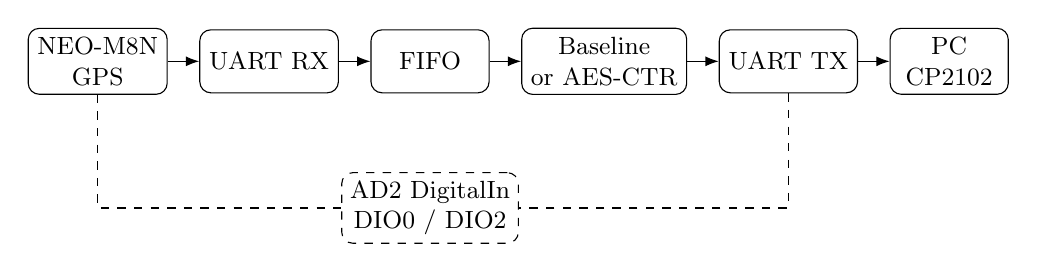
\begin{tikzpicture}[font=\small,>=Latex,node distance=7mm,
  box/.style={draw,rounded corners,align=center,minimum height=8mm,minimum width=15mm},
  tap/.style={draw,dashed,rounded corners,align=center,inner sep=3pt}]
\node[box] (gps) {NEO-M8N\\GPS};
\node[box,right=4mm of gps] (rx) {UART RX};
\node[box,right=4mm of rx] (fifo) {FIFO};
\node[box,right=4mm of fifo] (mode) {Baseline\\or AES-CTR};
\node[box,right=4mm of mode] (tx) {UART TX};
\node[box,right=4mm of tx] (pc) {PC\\CP2102};
\draw[->] (gps)--(rx);
\draw[->] (rx)--(fifo); \draw[->] (fifo)--(mode); \draw[->] (mode)--(tx); \draw[->] (tx)--(pc);
\node[tap,below=10mm of fifo] (ad2) {AD2 DigitalIn\\DIO0 / DIO2};
\draw[dashed] (gps.south) |- (ad2.west);
\draw[dashed] (tx.south) |- (ad2.east);
\end{tikzpicture}%
}
\caption{The two elaborations share the UART and FIFO path. During live trials, AD2 DIO0 samples GPS TX at FPGA RX and DIO2 samples FPGA TX; the CP2102 independently receives FPGA TX.}
\label{fig:architecture}
\end{figure}

The FIFO decouples UART reception from downstream handshakes. The framing error and FIFO overflow indicators are sticky. In the analyzed live trials, both indicators remained inactive and no reset was observed.

\subsection{AES-128-CTR}
For block index \(j\), AES encrypts a 128-bit counter block formed by appending a 32-bit counter to the 96-bit nonce. The counter is encoded in big-endian byte order. The resulting keystream block is XORed with the input bytes. The stream adapter advances its mask only when an output byte is accepted and prevents counter wraparound. The AES core computes a block in 20 cycles (400~ns at 50~MHz), with a documented 21-cycle issue interval. Current and held-next mask storage allow block computation to overlap UART reception, so mask generation can be scheduled ahead of byte transfer.

At 9600/8N1, a UART character occupies ten bit periods, approximately 1.042~ms. The 400~ns AES block computation is short relative to one serial character; this comparison describes scheduling headroom rather than measured end-to-end latency or throughput.

\begin{figure}[H]
\centering
\resizebox{\linewidth}{!}{%
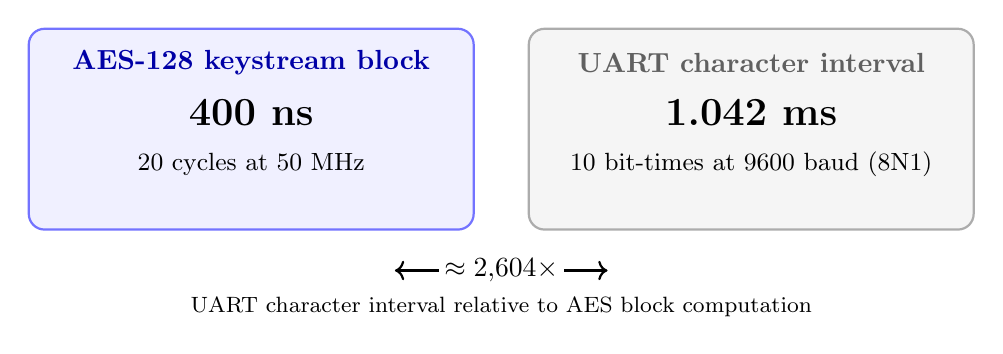
\begin{tikzpicture}[font=\small]
\draw[rounded corners=2mm,fill=blue!6,draw=blue!55,line width=0.8pt]
  (0,0) rectangle (5.65,2.55);
\draw[rounded corners=2mm,fill=gray!8,draw=gray!65,line width=0.8pt]
  (6.35,0) rectangle (12,2.55);
\node[font=\bfseries,color=blue!65!black] at (2.825,2.12) {AES-128 keystream block};
\node[font=\Large\bfseries] at (2.825,1.48) {400 ns};
\node at (2.825,0.83) {20 cycles at 50 MHz};
\node[font=\bfseries,color=gray!75!black] at (9.175,2.12) {UART character interval};
\node[font=\Large\bfseries] at (9.175,1.48) {1.042 ms};
\node at (9.175,0.83) {10 bit-times at 9600 baud (8N1)};
\draw[<->,line width=0.8pt] (4.65,-0.52)--(7.35,-0.52);
\node[fill=white,inner sep=2pt,font=\bfseries] at (6,-0.52) {\(\approx 2{,}604\times\)};
\node[font=\footnotesize,align=center] at (6,-0.98)
  {UART character interval relative to AES block computation};
\end{tikzpicture}%
}
\caption{The UART character interval is approximately 2,604 times the AES block-computation time at the selected operating point. This is a comparison of time scales, not a measurement of acceleration or effective throughput.}
\label{fig:prefetch}
\end{figure}

\section{Experimental Method}
\subsection{Verification Levels}
The evidence is separated into four levels: (1) RTL testbenches for AES, CTR, UART, FIFO, and integration; (2) independent Python decryption and NMEA validation; (3) Quartus post-fit resource and timing reports; and (4) physical DE10-Lite captures using AD2 and CP2102.

The AES regression contains 866 AES test-vector comparisons: 284 vectors from the NIST CAVP AES test set, six published examples, and 576 synthetic cases~\cite{CAVP}. These local regression checks do not constitute a formal NIST CAVP validation. Table~\ref{tab:kat} shows an AES-128 example from FIPS 197~\cite{FIPS197}. NIST SP 800-38A CTR examples are also exercised by the independent Python reference using the \texttt{cryptography} package (version 41.0.7 in the recorded run)~\cite{SP80038A}. The FIPS key is public test data, not a deployment secret; each live AES-CTR acquisition used a separate experimental key.

\begin{table}[H]
\caption{AES-128 known-answer example from FIPS 197.}
\label{tab:kat}
\centering
\small
\begin{tabular}{ll}
\hline
Field & Hexadecimal value \\
\hline
Key & \texttt{000102030405060708090a0b0c0d0e0f} \\
Plaintext & \texttt{00112233445566778899aabbccddeeff} \\
Expected ciphertext & \texttt{69c4e0d86a7b0430d8cdb78070b4c55a} \\
\hline
\end{tabular}
\end{table}

\subsection{Implementation and Physical Procedure}
The target is a DE10-Lite/MAX 10 \texttt{10M50DAF484C7G} with a 50~MHz clock, 9600/8N1 UART, and 1,024-byte FIFO. Matched baseline and AES-CTR builds use Quartus Prime 25.1, seed 1, and the same device and timing constraints. Source and build-artifact SHA-256 values were recorded alongside the post-fit metrics. Fmax is the minimum reported post-fit value across three timing corners; it is a static timing estimate, not a measured board frequency.

For live captures, the AD2 operated in DigitalIn mode as a two-channel logic analyzer, sampling GPS TX and FPGA TX simultaneously at 200,000 samples/s. The raw digital samples were decoded as UART frames and retained for frame-error checks and byte-level comparison; a CP2102 provided an independent host-side copy. The decoder reported zero framing errors and false starts on both lines, and the acquisition reported zero lost and corrupt samples. The GPS source was activated only after the capture setup confirmed that AD2 and CP2102 were armed, so both acquisitions covered the same stream. The baseline comparison checks GPS bytes directly against FPGA output. The AES-CTR comparison decrypts FPGA output starting from counter zero and checks all recovered bytes against the simultaneous GPS reference. CP2102 output is cross-checked against the AD2-decoded FPGA TX bytes.

The NMEA validator checks printable ASCII, line endings, sentence length, and checksums for complete sentences. Any incomplete edge fragments are retained in the byte-level comparison rather than trimmed.

\section{Results}
\subsection{Post-Fit Implementation Cost}
Table~\ref{tab:fit} reports the selected matched build pair. Both builds passed setup, hold, recovery, and removal checks in all three audited corners. Their worst slacks are positive at the 50~MHz operating clock. Adding AES increases logic and register use while reducing minimum Fmax; the AES-CTR fit nevertheless retains a substantial timing margin above the required clock.

\begin{table}[H]
\caption{Selected DE10-Lite post-fit metrics at 50~MHz and 9600/8N1.}
\label{tab:fit}
\centering
\small
\begin{tabular}{lrrr}
\hline
Metric & Baseline & AES-CTR & Change / check \\
\hline
Logic elements & \BaselineLE{} & \SecureLEPrint{} & +5,308 \\
Registers & \BaselineReg{} & \SecureReg{} & +701 \\
Memory bits & 8,192 & 8,192 & 0 \\
Pins & 14 & 14 & 0 \\
Minimum Fmax (MHz) & \BaselineFmax{} & \SecureFmax{} & $-27.93$ \\
Worst setup slack (ns) & 11.870 & 9.481 & Pass \\
Worst hold slack (ns) & 0.102 & 0.089 & Pass \\
Worst recovery slack (ns) & 14.454 & 13.184 & Pass \\
Worst removal slack (ns) & 0.439 & 2.216 & Pass \\
\hline
\end{tabular}
\end{table}

The AES-CTR design occupies 5,655 of the MAX 10's 49,760 LEs (11.36\%), compared with 347 LEs (0.70\%) for the baseline. Both use 8,192 memory bits, corresponding to the same FIFO capacity. These counts describe this RTL, Quartus flow, device, and selected fit.

\begin{figure}[H]
\centering
\resizebox{\linewidth}{!}{%
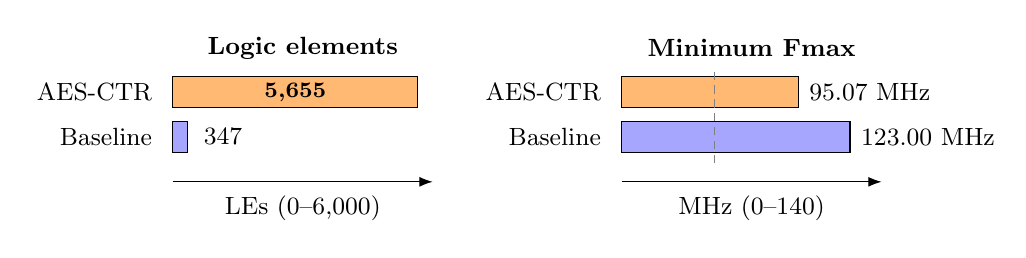
\begin{tikzpicture}[font=\small,>=Latex]
\pgfmathsetmacro{\BaselineLEBar}{3.3*(\BaselineLE/6000)}
\pgfmathsetmacro{\SecureLEBar}{3.3*(\SecureLE/6000)}
\pgfmathsetmacro{\BaselineFmaxBar}{3.3*(\BaselineFmax/140)}
\pgfmathsetmacro{\SecureFmaxBar}{3.3*(\SecureFmax/140)}
\pgfmathsetmacro{\ClockBar}{7.0+3.3*50/140}
\node[font=\small\bfseries] at (2.95,2.18) {Logic elements};
\node[font=\small\bfseries] at (8.65,2.18) {Minimum Fmax};
\node[anchor=east] at (1.16,1.62) {AES-CTR};
\node[anchor=east] at (1.16,1.05) {Baseline};
\draw[fill=orange!55] (1.3,1.42) rectangle ({1.3+\SecureLEBar},1.82);
\draw[fill=blue!35] (1.3,0.85) rectangle ({1.3+\BaselineLEBar},1.25);
% Keep the long value inside its bar, clear of the Fmax panel labels.
\node[font=\footnotesize\bfseries,inner sep=1pt] at ({1.3+\SecureLEBar/2},1.62) {\SecureLEPrint};
\node[anchor=west,fill=white,inner sep=1pt] at (1.65,1.05) {\BaselineLE};
\draw[->] (1.3,0.48)--(4.6,0.48);
\node[below] at (2.95,0.43) {LEs (0--6,000)};
\node[anchor=east] at (6.86,1.62) {AES-CTR};
\node[anchor=east] at (6.86,1.05) {Baseline};
\draw[fill=orange!55] (7.0,1.42) rectangle ({7.0+\SecureFmaxBar},1.82);
\draw[fill=blue!35] (7.0,0.85) rectangle ({7.0+\BaselineFmaxBar},1.25);
\node[anchor=west,fill=white,inner sep=1pt] at ({7.0+\SecureFmaxBar+0.1},1.62) {\SecureFmax{} MHz};
\node[anchor=west,fill=white,inner sep=1pt] at ({7.0+\BaselineFmaxBar+0.1},1.05) {\BaselineFmax{} MHz};
\draw[->] (7.0,0.48)--(10.3,0.48);
\node[below] at (8.65,0.43) {MHz (0--140)};
\draw[densely dashed,gray] (\ClockBar,0.72)--(\ClockBar,1.95);
\end{tikzpicture}%
}
\caption{Post-fit logic counts and minimum Fmax. The dashed marker in the Fmax panel indicates the 50~MHz operating clock.}
\label{fig:fit}
\end{figure}

\subsection{Live GPS Data-Path Results}
Table~\ref{tab:live} summarizes the paired 1,024-byte trials and supplementary 65,536-byte acquisitions. In the paired baseline and AES-CTR captures, each trial used a distinct live acquisition and compared exactly 1,024 bytes. Baseline FPGA output matched the simultaneous GPS reference; independent AES-CTR decryption matched its reference, and the CP2102 copy matched ciphertext decoded from AD2. Both paired trials had zero missing or extra bytes and no first-divergence offset; each contained 24 complete checksum-valid NMEA sentences. The separate 65,536-byte AES-CTR trial recovered the captured live GPS stream with byte-exact correspondence to the reference and contained 1,112 complete checksum-valid NMEA sentences. Incomplete edge fragments were retained in each byte-level comparison.

\begin{table}[H]
\caption{Simultaneous live GPS captures at 9600/8N1.}
\label{tab:live}
\centering
\small
\begingroup
\setlength{\tabcolsep}{3pt}
\begin{tabular}{@{}P{0.21\linewidth}P{0.14\linewidth}P{\dimexpr0.65\linewidth-4\tabcolsep\relax}@{}}
\hline
Mode & Bytes checked & Result \\
\hline
Baseline (paired) & 1,024 & Exact GPS-to-FPGA forwarding; 24 valid NMEA sentences \\
AES-CTR (paired) & 1,024 & Exact recovery after decryption; 24 valid NMEA sentences \\
AES-CTR (extended) & 65,536 & Exact recovery after decryption; 1,112 valid NMEA sentences \\
Baseline (supplementary) & 65,536 & All copies match byte-for-byte; NMEA rejects non-printable \texttt{0xEA} at offset 127 \\
\hline
\end{tabular}
\endgroup
\end{table}

For the paired AES-CTR trial, the ciphertext hash differed from the plaintext-reference hash, and its hash matched the CP2102 serial capture. The recovered hash equaled the simultaneous raw GPS reference hash. AD2 sampled both digital lines at 200~kS/s with no reported sample loss or corruption, and the UART decoder reported zero framing errors and false starts. In the extended AES-CTR capture, AD2 acquired 16,181,804 samples with zero lost or corrupt samples, decoded 65,536 frames on each channel, and reported zero framing errors or false starts. The ciphertext on AD2 and CP2102 had SHA-256 \SHA{88c96353f03e826e}{f9fa12001f21bd65}{6e5d70e277f31b25}{6e78e16cb3037328}; the recovered plaintext and GPS reference shared SHA-256 \SHA{84fc38de8c9fb9df}{25ce19b0489a6d73}{854ae07eb15876e2}{e01401c695f4bb2c}. The overflow and framing-error indicators remained inactive, and no reset was observed during the capture.

In the supplementary 65,536-byte baseline acquisition, the reference, FPGA output, and CP2102 files each had SHA-256 \SHA{337bd2fcee9c0577}{1b3319c73f26f16a}{3c7c5066e804d1a3}{d10c314a086d677d}. The comparison contained no missing or extra bytes and no first-divergence offset. AD2 reported zero lost or corrupt samples, zero framing errors, and zero false starts; the operator reported the overflow and framing indicators inactive and no reset. The strict NMEA validator nevertheless rejected the data because byte \texttt{0xEA} at offset 127 is not printable ASCII. Since that byte is present in the reference and all output copies, this run supports byte-transparent forwarding but is not counted as a clean NMEA capture. A focused follow-up could repeat the direct-source and integrated captures while checking GPS supply and UART input conditions; the present data do not establish the byte's origin.

\section{Discussion and Limitations}
Adding AES-CTR uses 5,308 more LEs and 701 more registers. Its 95.07~MHz minimum Fmax leaves a 45.07~MHz margin above the 50~MHz clock. The paired captures and the 65,536-byte AES-CTR capture matched their GPS references.

AES-CTR occupies 11.36\% of the MAX 10's 49,760 LEs, while the baseline occupies 0.70\%; both use the same 8,192 memory bits. These resource counts are specific to the selected device and Quartus fit.

At 9600/8N1, one UART character takes about 1.042~ms, compared with 400~ns per AES block and a 420~ns issue interval. This provides keystream scheduling margin at the tested rate; it is not an end-to-end latency measurement.

The supplementary baseline reference and output contain the same non-printable byte at offset 127: the path is byte-transparent, but the stream fails NMEA validation. The paired trials and extended AES-CTR capture pass both byte comparison and the NMEA checks in Table~\ref{tab:live}.

The 65,536-byte capture extends the live trial; repeated runs would be needed to characterize reliability. Fmax is derived from Quartus post-fit timing analysis.

AES-CTR provides confidentiality but not integrity, authenticity, or replay protection. The prototype loads the key and nonce as static build parameters; a deployed system would therefore require secure key provisioning, nonce management, and an authenticated mode or separate message-authentication mechanism.

\section{Conclusion}
This paper presents a controlled baseline-versus-AES-128-CTR implementation on a DE10-Lite/MAX 10 and evaluates post-fit cost and live GPS behavior at 50~MHz and 9600/8N1. The AES-CTR fit uses 5,655 LEs and 917 registers, compared with 347 LEs and 216 registers for the baseline design; its minimum Fmax is 95.07~MHz, with all audited timing slacks positive at the 50~MHz operating clock. Simultaneous live captures demonstrated exact baseline forwarding and AES-CTR recovery on paired 1,024-byte streams, plus exact recovery of a supplementary 65,536-byte AES-CTR stream. These results show that the evaluated AES-CTR datapath preserved the live GPS stream while meeting the target timing constraint.

\subsubsection{Acknowledgements.} The authors gratefully acknowledge the support of the Universidade do Estado do Amazonas (UEA) and the Laboratório de Sistemas Digitais e Microeletrônica (LSD$\mu$), coordinated by Prof. Edgard L. O. da Silva, for providing the institutional and technical environment that supported the development of this work.

\subsubsection{Declaration of AI-assisted technologies.} OpenAI ChatGPT and Codex assisted with manuscript drafting, language refinement, and editorial revision, as well as with developing and reviewing project scripts and experimental procedures. The authors conducted the hardware captures, reviewed the data and technical content, and take responsibility for the analyses and conclusions in the final manuscript.

\subsubsection{Competing interests.} The authors declare that they have no competing interests.

\begin{thebibliography}{9}
\raggedright

\bibitem{Abidin2020}
Abidin, Z., Aryawiratama, N., Muttaqin, A., Arisandi, E.D., Martineac, C.: Design of FPGA Based Data Parser for Global Positioning System. In: 2020 10th Electrical Power, Electronics, Communications, Controls and Informatics Seminar (EECCIS), pp. 159--162 (2020). \doi{10.1109/EECCIS49483.2020.9263455}

\bibitem{Majoral2023}
Majoral, M., Fern\'andez-Prades, C., Arribas, J.: A Flexible System-on-Chip Field-Programmable Gate Array Architecture for Prototyping Experimental Global Navigation Satellite System Receivers. Sensors \textbf{23}(23), 9483 (2023). \doi{10.3390/s23239483}

\bibitem{Prasanna2022}
Prasanna, T.L., Siddaiah, N., Krishna, B.M., Valluri, M.R.: Implementation of the Advanced Encryption Standard Algorithm on an FPGA for Image Processing Through the Universal Asynchronous Receiver-Transmitter Protocol. International Journal of Electrical and Computer Engineering \textbf{12}(6), 6114--6122 (2022). \doi{10.11591/ijece.v12i6.pp6114-6122}

\bibitem{Paz2024}
Ortiz Ni\~no, M.A., Paipilla Arenas, A.S., Paz Penagos, H.: Low Area Implementation of the Advanced Encryption Standard (AES) with Counter Mode (CTR) for System-On-Chip -- Field-Programmable Gate Array. Revista Elektr\'on \textbf{8}(2), 71--76 (2024). \doi{10.37537/rev.elektron.8.2.201.2024}

\bibitem{Visconti2020}
Visconti, P., Capoccia, S., Venere, E., Vel\'azquez, R., de Fazio, R.: 10 Clock-Periods Pipelined Implementation of AES-128 Encryption-Decryption Algorithm up to 28 Gbit/s Real Throughput by Xilinx Zynq UltraScale+ MPSoC ZCU102 Platform. Electronics \textbf{9}(10), 1665 (2020). \doi{10.3390/electronics9101665}

\bibitem{Azzouzi2025}
Azzouzi, O., Anane, M., Ghanem, M.C., Himeur, Y., Wojtczak, D.: Flexible and Area-Efficient Codesign Implementation of AES on FPGA. Cryptography \textbf{9}(4), 78 (2025). \doi{10.3390/cryptography9040078}

\bibitem{FIPS197}
National Institute of Standards and Technology: Advanced Encryption Standard (AES). FIPS PUB 197-upd1. NIST (2023). \doi{10.6028/NIST.FIPS.197-upd1}

\bibitem{SP80038A}
Dworkin, M.: Recommendation for Block Cipher Modes of Operation: Methods and Techniques. NIST Special Publication 800-38A. National Institute of Standards and Technology (2001). \doi{10.6028/NIST.SP.800-38A}

\bibitem{CAVP}
National Institute of Standards and Technology: Cryptographic Algorithm Validation Program: Block Ciphers. \url{https://csrc.nist.gov/projects/cryptographic-algorithm-validation-program/block-ciphers}. Accessed 30 September 2026

\end{thebibliography}
\end{document}
